\documentclass[10pt]{article}
\usepackage[ngerman]{babel}
\usepackage[utf8]{inputenc}
\usepackage[T1]{fontenc}
\usepackage{amsmath}
\usepackage{amsfonts}
\usepackage{amssymb}
\usepackage[version=4]{mhchem}
\usepackage{stmaryrd}
\usepackage{graphicx}
\usepackage[export]{adjustbox}
\graphicspath{ {./images/} }
\usepackage{bbold}

\title{Hauptprüfung Abiturprüfung 2023 - Leistungsfach }

\author{Alexander Schwarz\\
www.mathe-aufgaben.com}
\date{}


\begin{document}
\maketitle
 Baden-Württemberg\section*{Pflichtteil - Aufgabensatz 1}
\section*{Hilfsmittel: keine allgemeinbildende Gymnasien }


\section*{Aufgabe 1: (0,5 VP und 2 VP)}
Die Abbildung zeigt den Graphen der Funktion $f$ mit $f(x)=\sqrt{x+2}$ und die Gerade durch die Punkte A(2|2) und $B(3 \mid 0)$.\\
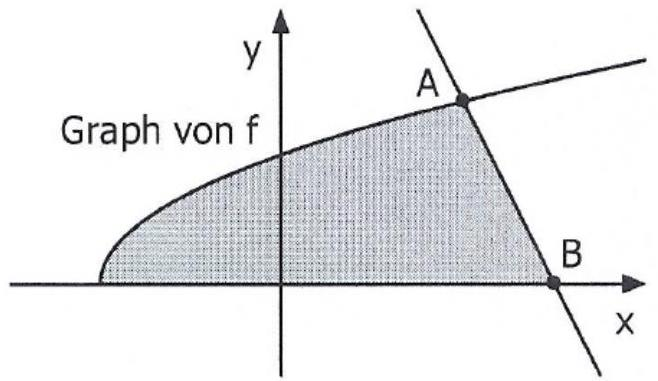
\includegraphics[max width=\textwidth, center]{2025_04_24_617d4790cd82121ee49eg-2(1)}\\
a) Geben Sie die maximale Definitionsmenge der Funktion $f$ an.\\
b) Bestimmen Sie den Inhalt der markierten Fläche.

\section*{Aufgabe 2: (1 VP und 1,5 VP)}
Die Abbildung in der Anlage zeigt den Graphen der in $\mathbb{R}$ definierten Funktion $f$, dessen einzige Extrempunkte $A(-1 \mid 1)$ und $B(0 \mid 0)$ sind, sowie den Punkt $P$.\\
a) Geben Sie die Koordinaten des Tiefpunkts des Graphen der in $\mathbb{R}$ definierten Funktion $g$ mit $g(x)=-f(x-3)$ an.\\
b) Der Graph einer Stammfunktion von $f$ verläuft durch P. Skizzieren Sie diesen Graphen in der Abbildung.

\section*{Aufgabe 3: (1 VP und 1,5 VP)}
Die Abbildung zeigt den Graphen einer in $\mathbb{R}$ definierten Funktion $f$.\\
a) Beurteilen Sie die folgende Aussage:\\
"Für jeden Wert von $x$ mit $0 \leq x \leq 2$ ist die Steigung des Graphen von $f$ kleiner als 3 ."\\
b) Mit dem Term $\pi \cdot \int_{0}^{2}(f(x))^{2} d x$ kann das Volumen eines Körpers berechnet werden. Begründen Sie,\\
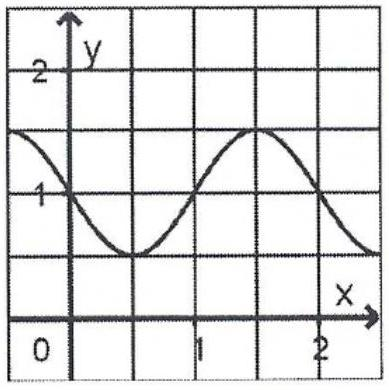
\includegraphics[max width=\textwidth]{2025_04_24_617d4790cd82121ee49eg-2} dass dieses Volumen größer als $\pi \cdot 0,5^{2}+\pi \cdot 1^{2}$ ist.

\section*{Aufgabe 4: (1 VP und 1,5 VP)}
Gegeben ist die Gerade $g: \vec{x}=\left(\begin{array}{l}0 \\ 1 \\ 1\end{array}\right)+t \cdot\left(\begin{array}{c}1 \\ 0 \\ -1\end{array}\right)$ mit $t \in \mathbb{R}$.\\
a) Zeigen Sie, dass $g$ in der Ebene $\mathrm{E}: \mathrm{x}_{1}+\mathrm{x}_{2}+\mathrm{x}_{3}=2$ liegt.\\
b) Gegeben ist außerdem die Schar der Geraden $h_{a}: \vec{x}=\left(\begin{array}{l}0 \\ 0 \\ 1\end{array}\right)+s \cdot\left(\begin{array}{l}1 \\ a \\ 0\end{array}\right)$ mit $s \in \mathbb{R}$ und $a \in \mathbb{R}$. Weisen Sie nach, dass $g$ und $h_{a}$ für jeden Wert von a windschief sind.

\section*{Aufgabe 5: (0,5 VP und 2 VP)}
Gegeben sind die Geraden $g: \vec{x}=\left(\begin{array}{l}1 \\ 1 \\ 1\end{array}\right)+r \cdot\left(\begin{array}{l}1 \\ 2 \\ 0\end{array}\right)$ und $\mathrm{h}: \overrightarrow{\mathrm{x}}=\left(\begin{array}{l}1 \\ 1 \\ 1\end{array}\right)+\mathrm{s} \cdot\left(\begin{array}{l}2 \\ 1 \\ 0\end{array}\right)$ mit $\mathrm{r}, \mathrm{s} \in \mathbb{R}$.\\
a) Begründen Sie , dass g und h nicht identisch sind.\\
b) Die Gerade g soll durch Spiegelung an einer Ebene auf die Gerade h abgebildet werden. Bestimmen Sie eine Gleichung einer geeigneten Ebene und erläutern Sie Ihr Vorgehen.

\section*{Aufgabe 6: (0,5 VP und 2 VP)}
In einem Behälter befinden sich fünf Kugeln, auf denen jeweils eine Zahl steht. Auf drei der Kugeln steht die Zahl 2, auf zwei der Kugeln die negative Zahl a. Zweimal nacheinander wird eine Kugel zufällig entnommen und wieder zurückgelegt.\\
a) Geben Sie im Sachzusammenhang ein Ereignis an, dessen Wahrscheinlichkeit mit dem Term $2 \cdot \frac{3}{5} \cdot \frac{2}{5}$ berechnet werden kann.\\
b) Die Zufallsgröße X gibt das Produkt der Zahlen an, die auf den beiden entnommenen Kugeln stehen. Der Erwartungswert von $X$ ist 4. Bestimmen Sie den Wert von a.

\section*{Abbildung zu Aufgabe 2 (Pflichtteil Aufgabensatz 1)\\}
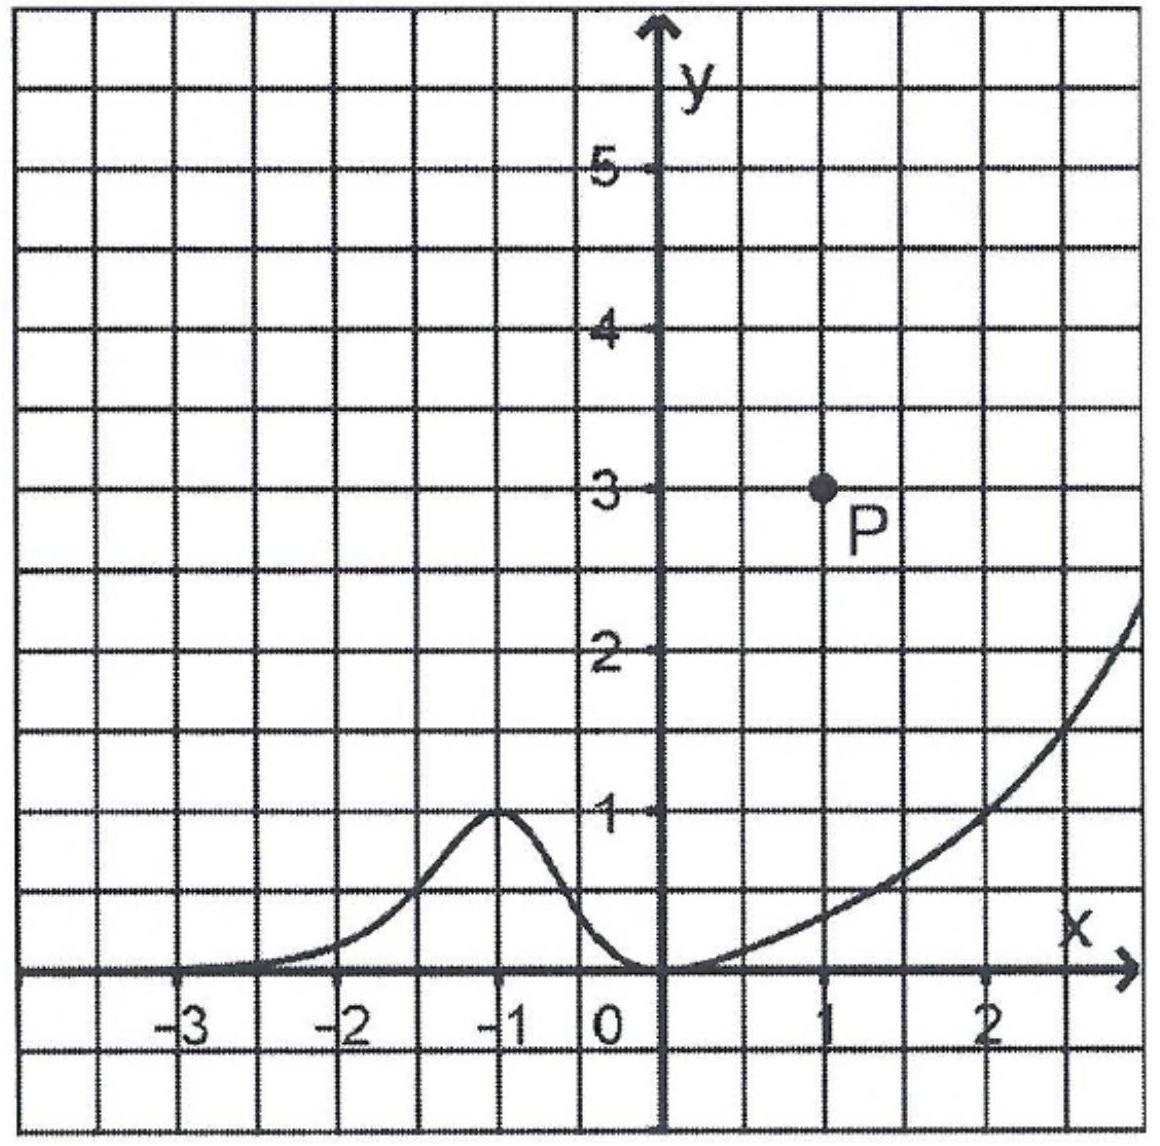
\includegraphics[max width=\textwidth, center]{2025_04_24_617d4790cd82121ee49eg-4}

\section*{Lösungen}
\section*{Aufgabe 1:}
a) maximale Definitionsmenge:

Bedingung: $x+2 \geq 0 \Leftrightarrow x \geq-2$\\
D $=[-2 ;+\infty[$\\
b)

Um den Flächeninhalt zu berechnen, muss die Fläche aufgeteilt werden.\\
Der linke Flächenteil kann mit Hilfe eines Integrals berechnet werden, der rechte Flächenteil ist ein Dreieck.\\
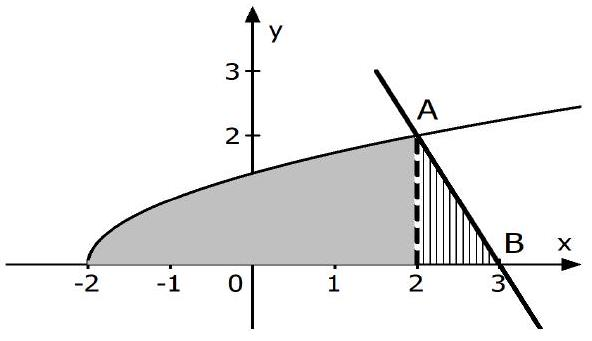
\includegraphics[max width=\textwidth, center]{2025_04_24_617d4790cd82121ee49eg-5}\\
$A_{\text {links }}=\int_{-2}^{2}(x+2)^{\frac{1}{2}} d x=\left[\frac{1}{3 / 2}(x+2)^{\frac{3}{2}}\right]_{-2}^{2}=\left[\frac{2}{3}(x+2)^{\frac{3}{2}}\right]_{-2}^{2}=\frac{2}{3} \cdot 4^{\frac{3}{2}}-0=\frac{2}{3} \cdot \sqrt{4^{3}}=\frac{16}{3}$\\
$\mathrm{A}_{\text {rechts }}=\mathrm{A}_{\text {Dreieck }}=\frac{1}{2} \cdot 1 \cdot 2=1$\\
$A_{\text {gesamt }}=\frac{16}{3}+1=\frac{19}{3} \mathrm{FE}$

\section*{Aufgabe 2:}
a) Das Schaubild von $g(x)=-f(x-3)$ ergibt sich aus dem Schaubild von $f$ durch eine Spiegelung an der x-Achse und einer anschließenden Verschiebung um 3 Längeneinheiten nach rechts.\\
Das Schaubild von $f$ besitzt den Hochpunkt H(-1|1).\\
Durch die Spiegelung an der x-Achse wird aus dem Hochpunkt ein Tiefpunkt mit den Koordinaten $\mathrm{T}(-1 \mid-1)$. Die anschließende Verschiebung um 3 LE nach rechts ergibt den gesuchten Tiefpunkt $\mathrm{T}^{*}(2 \mid-1)$.\\
b)

Erklärung:\\
An der Stelle x = 0 hat der Graph der\\
Stammfunktion einen Sattelpunkt, da der Graph von f dort eine Nullstelle ohne VZW besitzt.\\
Die Stammfunktion ist monoton wachsend, da sich der Graph von f oberhalb bzw. auf der $x$-Achse befindet.\\
Für $x \rightarrow-\infty$ nähert sich der Graph von $f$ der $x$-Achse an. Daher besitzt der Graph der Stammfunktion für $x \rightarrow-\infty$ eine waagrechte Asymptote.\\
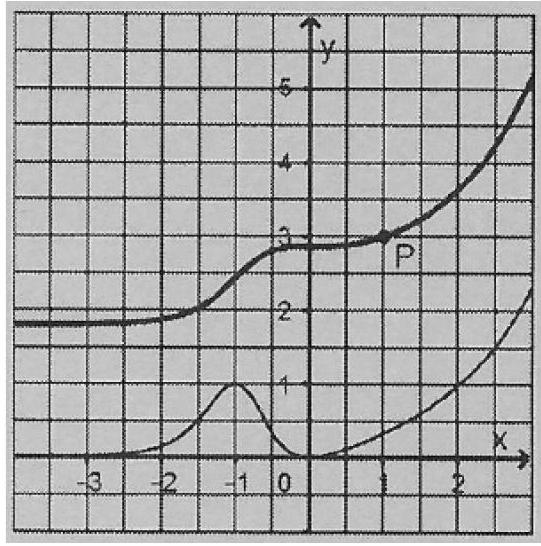
\includegraphics[max width=\textwidth, center]{2025_04_24_617d4790cd82121ee49eg-5(1)}

\section*{Aufgabe 3:}
a)

Aus der Abbildung kann man entnehmen, dass die Steigung des Graphen von f im Punkt $\mathrm{A}(1 \mid \mathrm{f}(1))$ am größten ist, da sich bei $x=1$ eine Wendestelle befindet.

Die Steigung der Tangente in diesem Punkt ist ca. 1,5 und damit kleiner als 3 .\\
Die Aussage ist richtig.\\
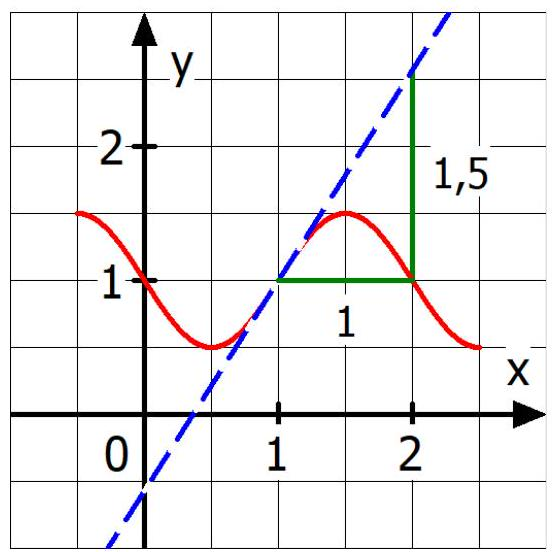
\includegraphics[max width=\textwidth, center]{2025_04_24_617d4790cd82121ee49eg-6}\\
b)

Der Term $\mathrm{V}^{*}=\pi \cdot \int_{0}^{2}(\mathrm{f}(\mathrm{x}))^{2} \mathrm{dx}$ gibt das Volumen des\\
Körpers an, der entsteht, wenn das Flächenstück, das der Graph von $f$ mit der x-Achse einschließt, um die x-Achse rotiert.

Interpretation des Terms $\pi \cdot 0,5^{2}$ :\\[0pt]
Rotiert das linke Rechteck im Intervall [0;1] um die $x$-Achse, entsteht ein Zylinder mit dem Volumen\\
$\mathrm{V}_{1}=\pi \cdot \mathrm{r}^{2} \cdot \mathrm{~h}=\pi \cdot 0,5^{2} \cdot 1=\pi \cdot 0,5^{2}$\\
Interpretation des Terms $\pi \cdot 1^{2}$ :\\
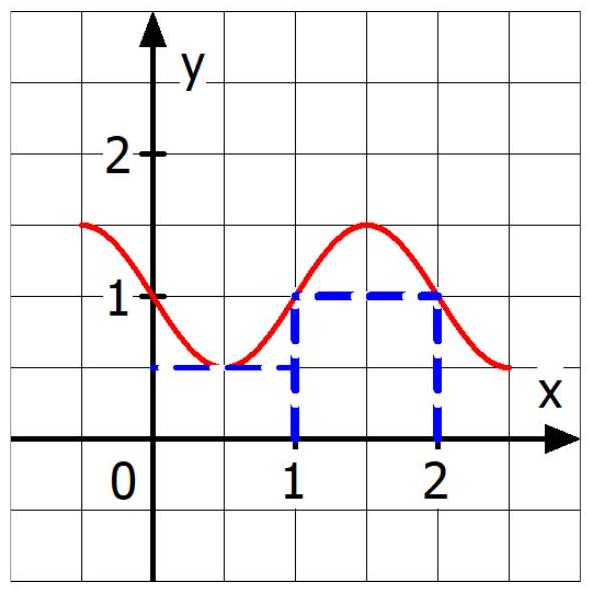
\includegraphics[max width=\textwidth, center]{2025_04_24_617d4790cd82121ee49eg-6(1)}

Rotiert das rechte Rechteck im Intervall [1;2] um die x-Achse, entsteht ein Zylinder mit dem Volumen $\mathrm{V}_{2}=\pi \cdot \mathrm{r}^{2} \cdot \mathrm{~h}=\pi \cdot 1^{2} \cdot 1=\pi \cdot 1^{2}$\\
Aus der Abbildung ergibt sich, dass die Summe der Zylindervolumen kleiner ist als das oben beschriebene Volumen $\mathrm{V}^{*}$.

\section*{Aufgabe 4:}
a) Aus der Geradengleichung kann aus den Zeilen entnommen werden:\\
$\mathrm{x}_{1}=\mathrm{t}$ und $\mathrm{x}_{2}=1$ und $\mathrm{x}_{3}=1-\mathrm{t}$\\
Einsetzen in die Ebenengleichung ergibt: $\mathrm{t}+1+(1-\mathrm{t})=2$\\
Daraus ergibt sich die wahre Aussage $2=2$.\\
Damit liegt g in der Ebene E .\\
b) Zunächst wird geprüft, ob die Richtungsvektoren für einen bestimmten Wert von a Vielfache sein können:\\
$\left(\begin{array}{l}1 \\ a \\ 0\end{array}\right)=k \cdot\left(\begin{array}{c}1 \\ 0 \\ -1\end{array}\right)$\\
Aus der 1.Zeile ergibt sich $\mathrm{k}=1$.\\
Aus der 3.Zeile ergibt sich $0=-1$, also ein Widerspruch.\\
Somit sind die Richtungsvektoren für jeden Wert von a keine Vielfache zueinander.

Gleichsetzen der Geradengleichungen:\\
$\left(\begin{array}{l}0 \\ 0 \\ 1\end{array}\right)+s \cdot\left(\begin{array}{l}1 \\ a \\ 0\end{array}\right)=\left(\begin{array}{l}0 \\ 1 \\ 1\end{array}\right)+t \cdot\left(\begin{array}{c}1 \\ 0 \\ -1\end{array}\right)$\\
3.Zeile: $1=1-\mathrm{t} \Leftrightarrow \mathrm{t}=0$\\
1.Zeile: $s=t \Rightarrow s=0$\\
2.Zeile: $s \cdot a=1 \Rightarrow 0 \cdot a=1$ ergibt einen Widerspruch

Das Gleichungssystem ist nicht lösbar, daher sind die Geraden für jeden Wert von a windschief.

\section*{Aufgabe 5:}
a) Die Geraden können nicht identisch sein, da ihre Richtungsvektoren keine Vielfachen zueinander sind.\\
b) Da die Stützvektoren der Geraden identisch sind, schneiden sich die Geraden im Punkt S(1|1|1).\\
Dieser Punkt muss auch auf der Spiegelebene liegen.\\
Es gibt zwei Möglichkeiten, den Normalenvektor der Ebene zu erhalten:\\
1.Möglichkeit:

Zunächst werden die beiden Richtungsvektoren skizziert, die in der $\mathrm{x}_{1}-\mathrm{x}_{2}$-Ebene liegen.\\
Der Normalenvektor von E halbiert den Winkel zwischen den Richtungsvektoren.\\
Die Richtungsvektoren besitzen dieselbe Länge, es gilt $\left.\left\lvert\, \begin{array}{l}2 \\ 1 \\ 0\end{array}\right.\right)\left|=\left|\left(\begin{array}{l}1 \\ 2 \\ 0\end{array}\right)\right|=\sqrt{5}\right.$.\\
Der Normalenvektor ist $\overrightarrow{\mathrm{n}}=\left(\begin{array}{l}2 \\ 1 \\ 0\end{array}\right)+\left(\begin{array}{l}1 \\ 2 \\ 0\end{array}\right)=\left(\begin{array}{l}3 \\ 3 \\ 0\end{array}\right)$ bzw. $\overrightarrow{\mathrm{n}^{*}}=\left(\begin{array}{l}1 \\ 1 \\ 0\end{array}\right)$.\\
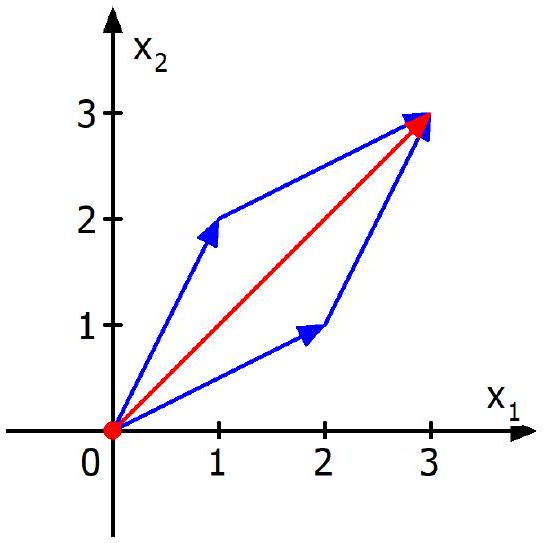
\includegraphics[max width=\textwidth, center]{2025_04_24_617d4790cd82121ee49eg-8(1)}

Ansatz für die Ebenengleichung: $x_{1}+x_{2}=d$\\
Einsetzen von $S(1|1| 1)$ ergibt $d=2$.\\
Die Gleichung der Ebene lautet $\mathrm{x}_{1}+\mathrm{x}_{2}=2$\\
2.Möglichkeit:

Zunächst werden die beiden Richtungsvektoren skizziert, die in der $\mathrm{x}_{1}-\mathrm{x}_{2}$-Ebene liegen, wobei der Vektor $\left(\begin{array}{l}1 \\ 2 \\ 0\end{array}\right)$ durch den Gegenvektor $\left(\begin{array}{c}-1 \\ -2 \\ 0\end{array}\right)$ ersetzt wird.

Der Normalenvektor von E halbiert den Winkel zwischen den Richtungsvektoren.\\
Die Richtungsvektoren besitzen dieselbe Länge, es gilt $\left.\left\lvert\, \begin{array}{l}2 \\ 1 \\ 0\end{array}\right.\right)\left|=\left|\left(\begin{array}{c}-1 \\ -2 \\ 0\end{array}\right)\right|=\sqrt{5}\right.$.\\
Der Normalenvektor ist $\overrightarrow{\mathrm{n}}=\left(\begin{array}{l}2 \\ 1 \\ 0\end{array}\right)+\left(\begin{array}{c}-1 \\ -2 \\ 0\end{array}\right)=\left(\begin{array}{c}1 \\ -1 \\ 0\end{array}\right)$.\\
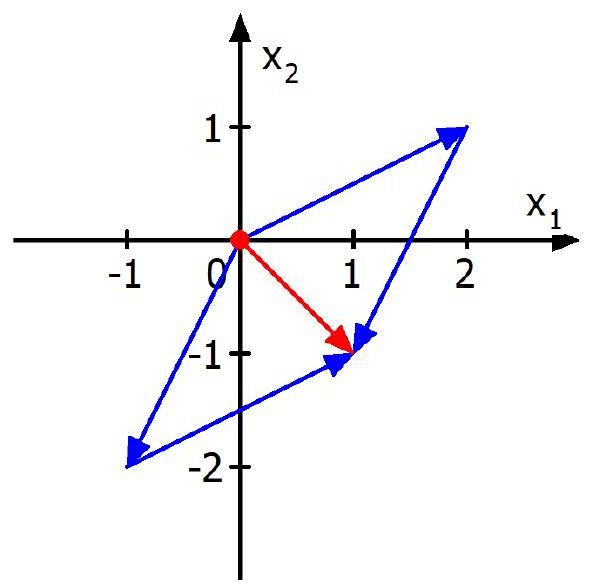
\includegraphics[max width=\textwidth, center]{2025_04_24_617d4790cd82121ee49eg-8}

Ansatz für die Ebenengleichung: $x_{1}-x_{2}=d$\\
Einsetzen von $\mathrm{S}(1|1| 1)$ ergibt $\mathrm{d}=0$.\\
Die Gleichung der Ebene lautet $\mathrm{x}_{1}-\mathrm{x}_{2}=0$

\section*{Aufgabe 6:}
a) $\frac{3}{5}$ ist die Wahrscheinlichkeit für die Ziehung von „2".\\
$\frac{2}{5}$ ist die Wahrscheinlichkeit für die Ziehung von „a".\\
$2 \cdot \frac{3}{5} \cdot \frac{2}{5}$ ist die Wahrscheinlichkeit, dass auf den beiden Kugeln unterschiedliche Zahlen stehen.\\
b) Die Zufallsgröße X kann folgende Werte annehmen:\\
$X=2 \cdot 2=4$ und $X=a \cdot a=a^{2}$ und $X=2 \cdot a$.\\
$\mathrm{P}(\mathrm{X}=4)=\frac{3}{5} \cdot \frac{3}{5}=\frac{9}{25}$\\
$P\left(X=a^{2}\right)=\frac{2}{5} \cdot \frac{2}{5}=\frac{4}{25}$\\
$P(X=2 a)=2 \cdot \frac{2}{5} \cdot \frac{3}{5}=\frac{12}{25}$\\
$E(X)=4 \cdot \frac{9}{25}+a^{2} \cdot \frac{4}{25}+2 a \cdot \frac{12}{25}=\frac{4}{25} a^{2}+\frac{24}{25} a+\frac{36}{25}$\\
Bedingung: $\left.\frac{4}{25} a^{2}+\frac{24}{25} a+\frac{36}{25}=4 \quad \right\rvert\, \cdot 25$

$$
4 a^{2}+24 a+36=100 \quad \mid: 4
$$

$$
a^{2}+6 a+9=25 \Leftrightarrow a^{2}+6 a-16=0
$$

$$
a_{1,2}=\frac{-6 \pm \sqrt{36+64}}{2}=\frac{-6 \pm 10}{2}
$$

Es gilt $a_{1}=-8$ und $a_{2}=2$.\\
Da a negativ ist, gilt a = -8.


\end{document}